\chapter{Volba a návrh periferií}
    Tato kapitola se již věnuje návrhu konkrétních periferií, tedy jednotlivých senzorů a akčních členů. Po technické stránce jsou všechny zmíněné moduly nadstavbou pro \uv{obecný modul periferie} popsaný detailně v předešlé kapitole. Jelikož je celý systém modulární, je pravděpodobné, že postupem času bude dále rozšiřován o nové typy periferií a i v současné chvíli je jich v plánu více, než je v možnostech této práce. Pro lepší přehlednost se v tab.\ref{tab:prehled-periferii} nachází přehled všech realizovaných i v tuto chvíli pouze plánovaných periferií.

    \begin{table}[h]
        \centering
        \caption{Přehled periferií.}
        \label{tab:prehled-periferii}
        \begin{tabular}{|l|l|l|l|l|}
            \hline
            Název & Typ & Napájení & Měřené / ovládané veličiny & Realizováno \\ \hline\hline
            Sensor teploty  & S & \qty{5}{V}    & Teplota vody                       & Ano, kap.~\ref{sec:perif-sensor-teploty}  \\ \hline
            Sensor hladiny  & S & \qty{5}{V}    & Výška hladiny (spojitě + skokově)  & Ano, kap.~\ref{sec:perif-sensor-hladina}  \\ \hline
            LED osvětlení   & A & \qty{24}{V}   & Intenzita osvětlení                & Ano, kap.~\ref{sec:perif-led-osvetleni}  \\ \hline
            Sensor pH       & S & \qty{5}{V}    & pH vody                            & Ano, kap.~\ref{sec:perif-sensor-ph}  \\ \hline
            Topné těleso    & A & \qty{230}{V}  & Ohřev vody                         & Ano, kap.~\ref{sec:perif-230v}  \\ \hline
            Filtr vody      & S & \qty{230}{V}  & Filtrace vody                      & Ano, kap.~\ref{sec:perif-230v}  \\ \hline
            Krmítko         & A & \qty{24}{V}   & Dávkování krmiva                   & N  \\ \hline
            Sensor průtoku  & S & -             & Voda tekoucí filtrem               & N  \\ \hline
                            & S &  &  & A  \\ \hline
                                & S &  &  & A  \\ \hline
                                & S &  &  & A  \\ \hline
                                & S &  &  & A  \\ \hline
                                & S &  &  & A  \\ \hline
                                & S &  &  & A  \\ \hline
                                & S &  &  & A  \\ \hline
                                & S &  &  & A  \\ \hline
                                & S &  &  & A  \\ \hline
            \end{tabular}
        
    \end{table}
    % TODO zkontrolovat styl vuci sablone prace

\section{LED osvětlení}
\label{sec:perif-led-osvetleni}

\section{Senzor teploty}
\label{sec:perif-sensor-teploty}

\section{Senzor výšky hladiny}
\label{sec:perif-sensor-hladina}

\section{Senzor pH}
\label{sec:perif-sensor-ph}

\section{Ovládání 230V periferií}
\label{sec:perif-230v}
%    \textit{    TODO: vybrán GPIO expandér (https://www.laskakit.cz/pcf8574-i2c-8bit-i-o-expander) a relé modul, řízeno přímo z ESP32 -- je to v jedné krabici, tak je zbytečně složité tam dávat další MCU. } 

Jak vyplývá z~požadavků zařízení a přehledu používané akvaristické techniky, pro automatizovaný provoz akvária je nutné umožnit řídící jednotce ovládat několik okruhů se síťovým napětím a spínat tak zvlášť zakoupené hotové spotřebiče pracující s~tímto napětím. Jedná se typicky o~ohřev vody, filtr, popř. některé druhy osvětlení. 

\begin{figure}[h!]
    \centering
    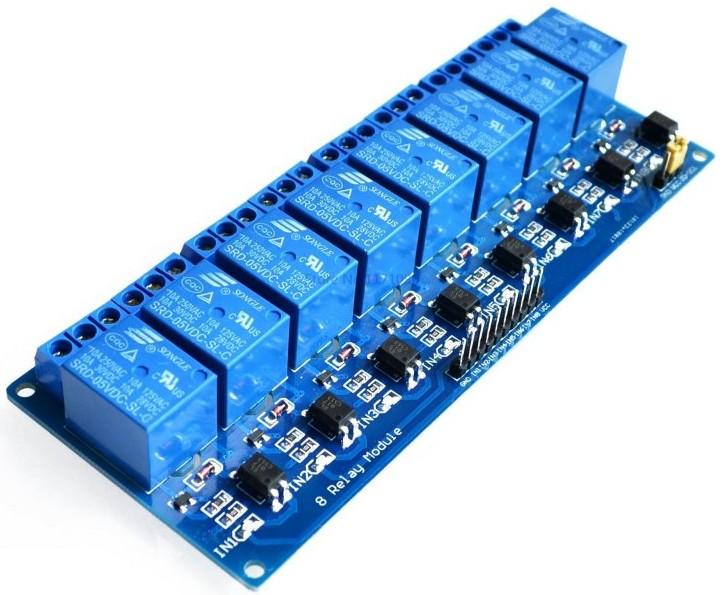
\includegraphics[width=0.6\textwidth]{obrazky/230/rele.jpg}
    \caption{Relé modul, ilustrační foto. Převzato z~\cite{eshop-laskakit-rele}.}
    \label{fig:obrazky-230-rele-jpg}
\end{figure}

\begin{figure}[h!]
    \centering
    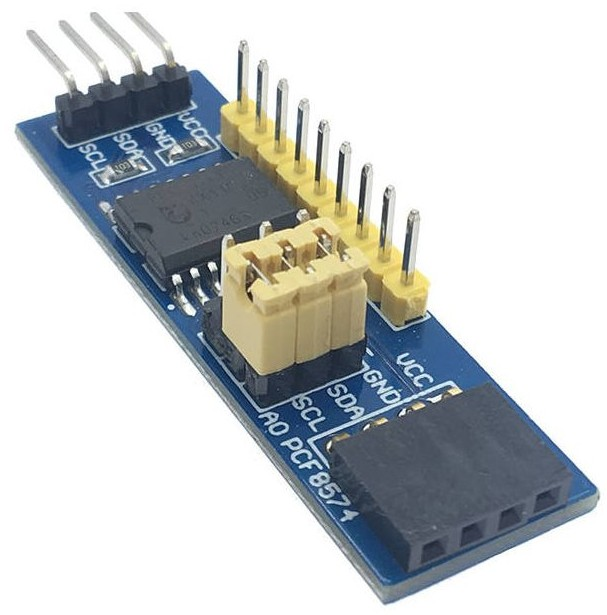
\includegraphics[width=0.4\textwidth]{obrazky/230/expander.jpg}
    \caption{Modul expandéru GPIO pinů, ilustrační foto. Převzato z~\cite{eshop-laskakit-expander}.}
    \label{fig:obrazky-230-expander-jpg}
\end{figure}

Aby uživatel mohl zařízení bezpěčně zapojit bez nutnosti odborné způsobilosti, budou se na hlavním šasi zařízení nacházet čtyři standartní zásuvky (typ E) s~jednofázovým napětím \qty{230}{V}. Fázové vodiče budou uvnitř zařízení přerušeny spínacími relé. Bude použit předpřipravený modul disponující osmi relé,kupříkladu modul na obr.~\ref{fig:obrazky-230-rele-jpg}. Zbylé čtyři relé slouží jako rezerva pro případ poškození některého z~používaných relé nebo při potřebě rozšíření o~další zásuvky. 

Z~důvodu nedostatku pinů na mikrokontroleru řídící jednotky (ESP32) bude k~relé modulu připojen ještě jeden externí modul a to expandér GPIO pinů komunikující přes sběrnici \acs{i2c}~\cite{eshop-laskakit-expander}, ilustrační foto na obr.~\ref{fig:obrazky-230-expander-jpg}. Z~pohledu mikrokontroleru tak budou všechny \qty{230}{V} zásuvky řízeny pomocí dvou datových pinů (SDA, SCL), které je navíc možné dále využít pro připojení jiných periferií jako např. OLED displaye pro zobrazení stavu zařízení. 

Možným zlepšením a rozšířením práce by bylo také zahrnutí obou zmíněných modulů přímo na DPS řídící jednotky. 


